\documentclass{VUMIFInfKursinis}
\usepackage{algorithmicx}
\usepackage{algorithm}
\usepackage{algpseudocode}
\usepackage{amsfonts}
\usepackage{amsmath}
\usepackage{bm}
\usepackage{color}
% \usepackage{hyperref}  % Nuorodų aktyvavimas
\usepackage{url}


% Titulinio aprašas
\university{Vilniaus universitetas}
\faculty{Matematikos ir informatikos fakultetas}
\department{Programų sistemų katedra}
\papertype{Kursinis darbas}
\title{Gestų kalbos atpažinimas naudojant internetinę kamerą}
\titleineng{Sign language recognition using web camera}
\status{3 kurso I grupės studentas}
\author{Pranciškus Ambrazas}
\supervisor{asist. Linas Petkevičius}
\date{Vilnius, \the\year}

% Nustatymai
% \setmainfont{Palemonas}   % Pakeisti teksto šriftą į Palemonas (turi būti įdiegtas sistemoje)
\bibliography{bibliografija} 

\begin{document}
\maketitle

\tableofcontents

\sectionnonum{Įvadas}
Daugiau nei 360 milijonų žmonių pasaulyje kenčia dėl klausos ir kalbos įvairių problemų, o daugiau nei 32 milijonai jų yra vaikai ir šis skaičius vis auga \cite{WhoInt}. Gestų kalba yra pagrindinis šių žmonių bendravimo įrankis. Tačiau reiktų pastebėti ir tai, jog dalis jų moka skaityti iš lūpų. Norint žmogui be šių ydų bendrauti su gestakalbiu (\textit{gestų kalba kalbantis žmogus}) reikia vertėjo, kuris išverstų gestų kalbą į įprastinę ir atvirkščiai.

Kiekviena pasaulyje esanti kalba turi ir savo gestų kalbą.Tai reiškia, skiriasi tiek gestų kalbos gramatika, tiek netgi patys gestai. Pasaulyje randama net dialektų pagal regionus, ne tik pagal šalis. Pavyzdžiui, amerikiečių anglų kalba šnekančių žmonių pasaulyje yra apie 500 tūkstančių \cite{remiantis United States Census Bureau’s data from the 2009-2013 American Community Survey}. Todėl netgi bendraujant dviem žmonėms, mokantiems gestų kalbą neretai iškyla vertimo problema, tad tenka ieškoti gestų vertimų. Paiešką galima atlikti atsižvelgiant į delno padėtį, rankos judesį (ar net abiejų rankų), rankos padėtį ir kiek rankų atlieka gestą. Tuomet pagal gesto išvaizdos paveiksliukus ar kartais net vaizdo įrašus, gestakalbiai gali išsiversti gestus. Tam yra skirtos tiek internetinės svetainės - žodynai, tiek įvairūs rašytiniai žodynai.

Šio tyrimo tikslas - padėti ne tik gestakalbiams tarpusavyje, bet ir žmonėms, nesuprantantiems gestų kalbos bendrauti su gestakalbiais tam pasitelkiant technologijas, taip suteikiant šiems žmonėms pilnavertį gyvenimą bendraujant su kitais. Šiuo tyrimu siekiama apžvelgti ir įvertinti ar naudojantis įprasta kompiuterine kamera įmanoma paversti gestų kalbą rašytiniu tekstu ar net garsine kalba ir lygiai taip pat versti rašytinę ar garsinę kalbą į gestų kalbą. Taip pat siekiama, kad vėliau būtų sukurtas visiems gestakalbiams prieinamas produktas ar programinė įranga, kurią kiekvienas įsidiegęs į savo įrenginį - kompiuterį, mobilųjį telefoną ar planšetinį kompiuterį galėtų naudotis šiuo vertėju. Taip pat tai galėtų tapti ir mokomąja gestų kalbos priemone. 

Šiuo metu yra gaminamas vienas iš tokių produktų, tačiau tai yra atskiras įrenginys, turintis įmontuotą kamerą, kuri be vaizdo taip pat fiksuoja ir atstumą iki tam tikrų objektų (šiuo atveju rankos), tačiau produkto kūrėjai sako, jog jų įrenginys galės versti gestų kalbą į anglų ir kitas kalbas ir lygiai taip pat versti įprastą kalbą į rašytinę kalbą. Plačiau: \textit{http://www.motionsavvy.com/}

Šiame darbe bus pagrinde nagrinėjama amerikiečių (\textit{angl. American Sign Language (ASL)}) ir lietuvių gestų kalbos.
%Įvade apibūdinamas darbo tikslas, temos aktualumas ir siekiami rezultatai.
%Darbo įvadas neturi būti dėstymo santrauka. Įvado apimtis 1–2 puslapiai.

\section{Teorija}
Šiame skyriuje bus aprašoma teorija apie apsimokančias sistemas ir neuroninius tinklus

\subsection{Savaime apsimokančios sistemos}
\textbf{Apsimokančios sistemos} (\textit{angl. machine learning}) - tai mokslas apie tai, kaip kompiuterius užprogramuoti taip, jog jie patys darytų sprendimus be žmogaus įsikišimo neužprogramuojant kiekvienos galimos situacijos. Kitais žodžiais tariant, leisti kompiuteriui pačiam nuspręsti kaip elgtis esant tam tikroms aplinkybėms. Savaime apsimokančios sistemos yra didelis žingsnis į priekį norint sukurti dirbtinį intelektą.

Savaime apsimokančių sistemų ir jų algoritmų sukūrimo dėka gatvėmis pradėjo važinėti patys save vairuojantys automobiliai (\textit{angl. self-driving cars}) arba dar kitaip vadinamos autonominės transporto priemonės. Įvairūs paieškos varikliai tokie kaip „Google“ ar „Yahoo“ taikydami šiuos alogirtmus naudotojams rodo kiekvienam asmeniškai sugeneruotą turinį. Taip pat reikėtų paminėti ir kalbos atpažinimo sistemas tokias kaip „Siri“ ar „Google Assistant“, kurios iš joms duotų komandų atlieka tam tikrus veiksmus.

\subsection{Neuroniniai tinklai}
Neuroniniai tinklai buvo sukurti atsižvelgiant į žmogaus smegenų struktūrą. Žmogaus smegenis sudaro neuronai. Atskirai neurodas atlieka įvairius veiksmus ir skaičiavimus ir perduoda elektrinius impulsus kitiems neuronams. Esant neuroniniam tinklui, jiems sąveikaujant tarpusavyje, smegenys tam tikrus veiksmus atlieka daug kartų greičiau nei kompiuteriai. Tai galima pagrįsti tuo, kad neuronas perduoda savo vienam iš kaimynų impulsą, ta kryptimi, kuria reikalauja atėjęs impulsas. Todėl žmonės pajautę karštį patraukia rankas.


\subsubsection{Dirbtiniai neuroniniai tinklai}
\textbf{Dirbtinis neuroninis tinklas} (\textit{angl. Artificial neural network}) - struktūra, skirta apdoroti dideliam kiekiui informacijos, sukurta rementis žmogaus nervų sistemos veikimo principu.

Šiam dideliam informacijos kiekiui apdoroti yra komponentai, atliekantys tam tikrus skaičiavimus, dar vadinami neuronais. Vienas neuronas yra tarpusavyje sujungtas su dar daugybe kitų. Atėjus signalui, neuronai perduoda informaciją vienas kitam, kol galiausiai pasiekiamas tam tikras veiksmas, kurį reikia atlikti. Tam kad signalas keliautų teisingu keliu, reikia, kad jungtys tarp neuronų būtų užtektinai stiprios. Tam, dirbtiniuose neuronų tinkluose yra pasitelkiamos savaime apsimokančios sistemos.


\subsubsection{Rekurentiniai neuroniniai tinklai}
\textbf{Rekurentiniai neuroniniai tinklai} (\textit{angl. Recurrent neural network}) - tai dirbtinis neuroninis tinklas, kuris saugo informaciją apie praeituose žingsniuose (neuronuose) atliktus veiksmus ar skaičiavimus.

\begin{figure}[H]
	\centering
	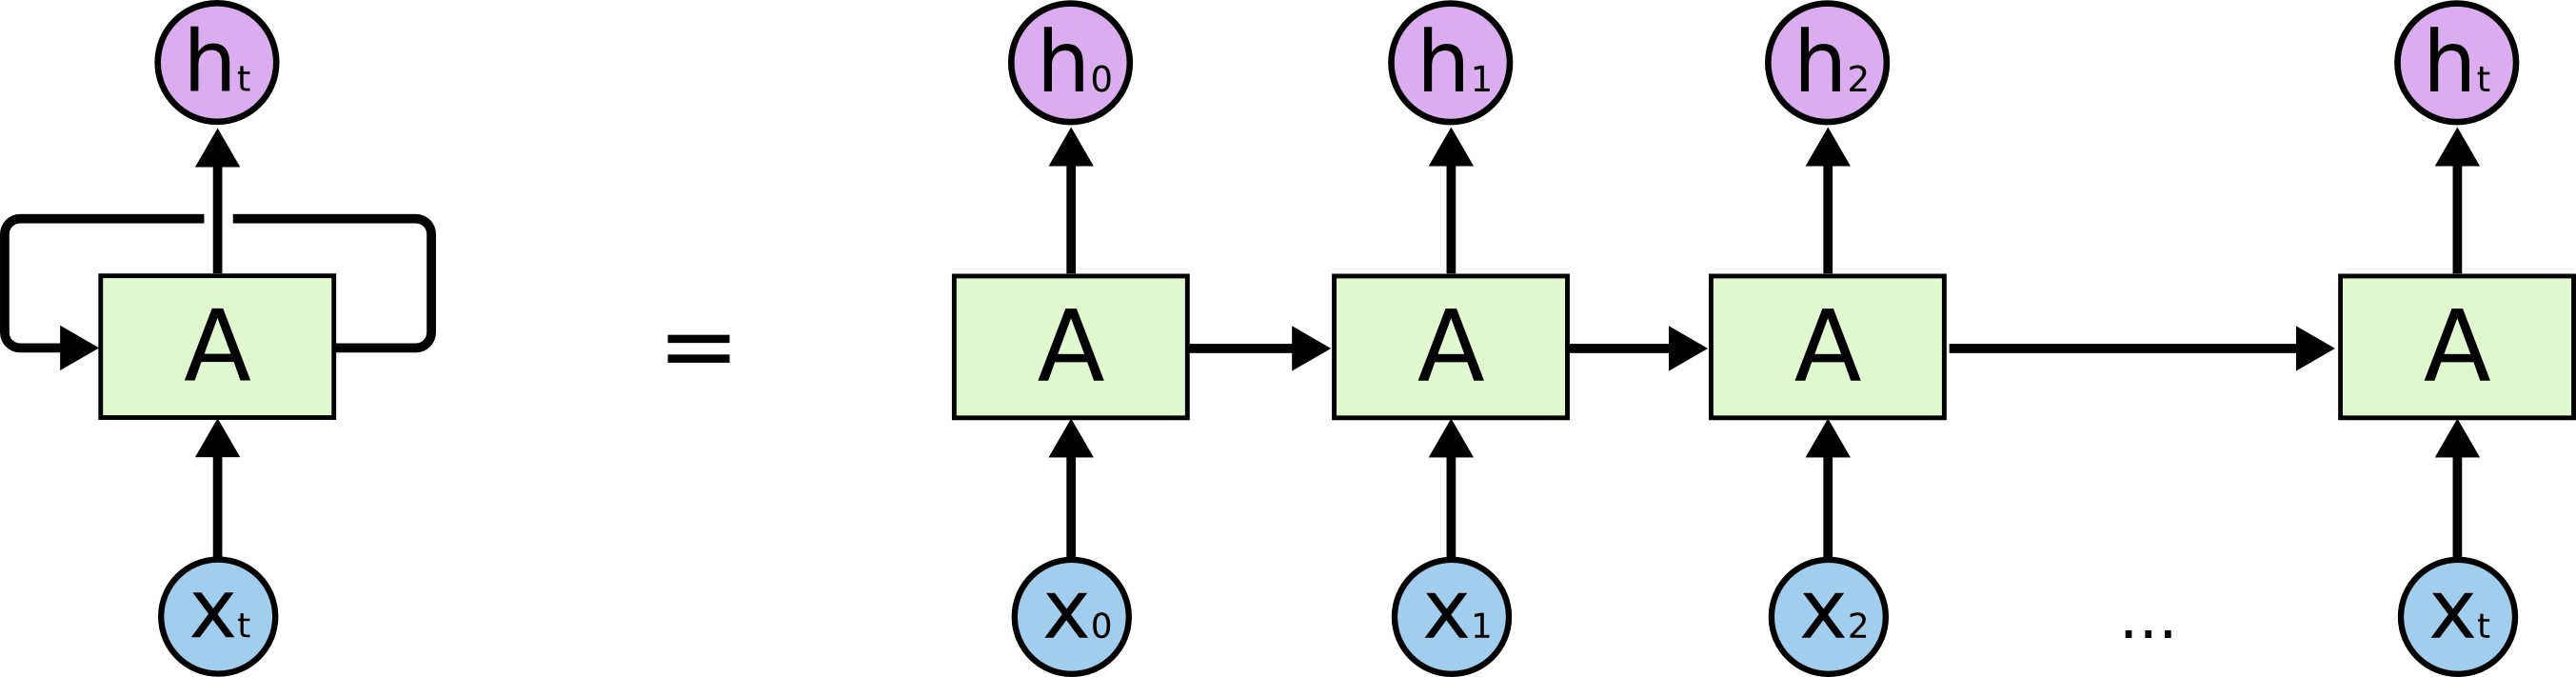
\includegraphics[width=.8\linewidth]{img/rnn}
	\caption{Rekurentinių neuroninių tinklų schema \cite{RecurrentNeuralNetwork}}
	\label{img:rnn}
	
\end{figure}
\begin{itemize}
	\item \textit{x\textsubscript{t}} - įeiga momentu \textit{t}
	\item \textit{h\textsubscript{t}} - išeiga momentu \textit{t}	
	\item \textit{A\textsubscript{t}} - būsena momentu \textit{t}	
\end{itemize}




\section{Gestų kalba}
\subsection{Gestų kalbos skirstymas}
Gestų kalba susideda iš dviejų dalių - statinių ir dinaminių ženklų. Gestų kalboje kiekviena kalba turi savo abėcėlę. Statiniais ženklais atvaizduojama didžioji abėcėlių raidžių dalis. O dinaminiais - žodžiai ir kai kurios gestų abėcėlių raidės. \textit{Pavyzdžiui}, amerikiečių gestų kalbos abėcėlėje J ir Z raidės atvaizduojamos dinaminiais judesiais (\textit{žr. \ref{img:asl_alphabet} pav.}), o lietuvių - Ą, D, Į, K ir kt. bei jau minėtosios J ir Z raidės (\textit{žr. \ref{img:lsl_alphabet} pav.})

\begin{figure}[H]
	\centering
	\begin{minipage}{.5\textwidth}
		\centering
		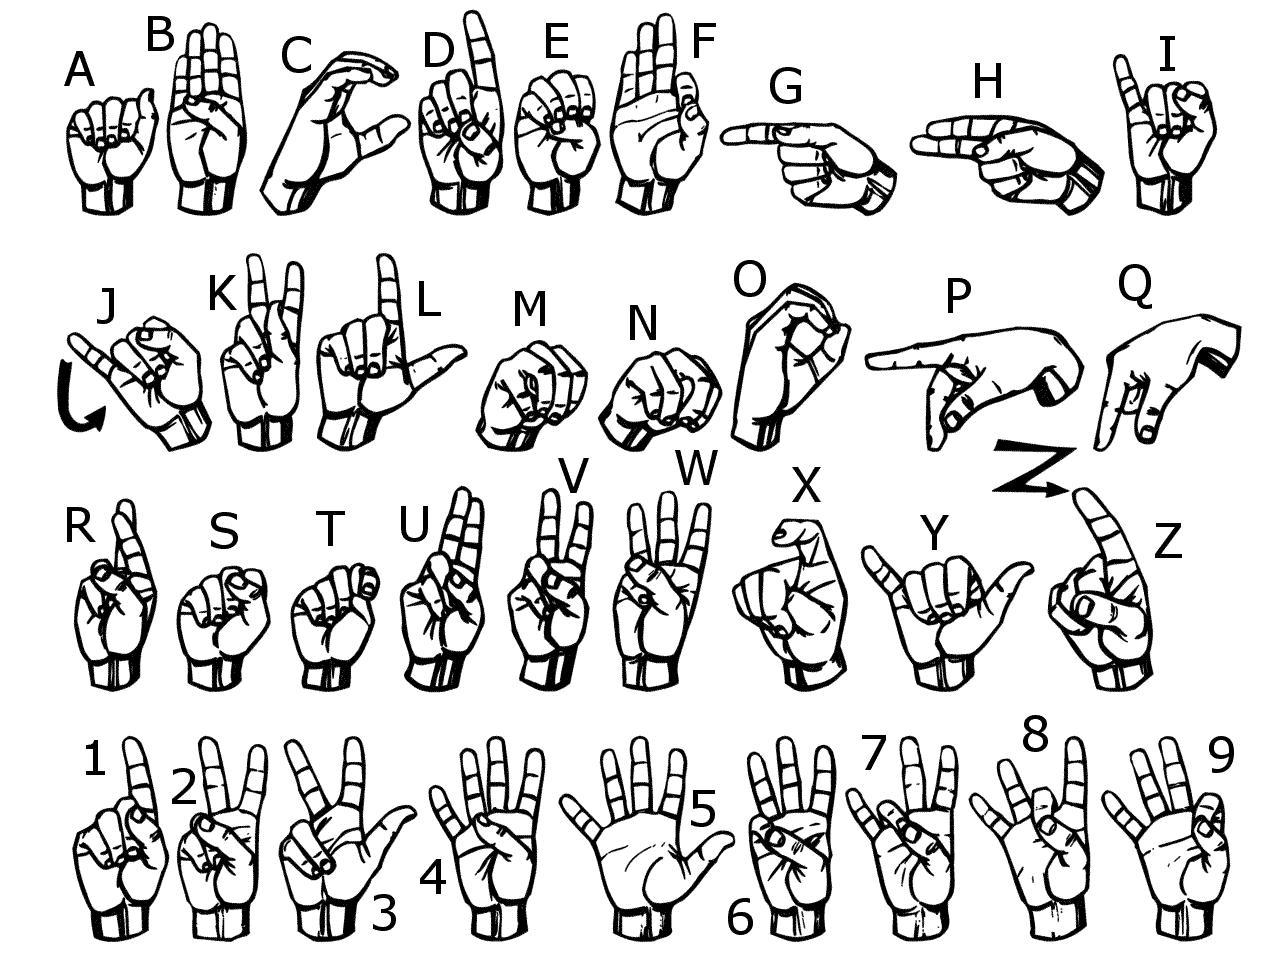
\includegraphics[width=.8\linewidth]{img/asl_alphabet}
		\caption{Amerikiečių gestų kalbos abėcėlė}
		\label{img:asl_alphabet}
		%http://lifeprint.com/asl101/topics/wallpaper1.htm
	\end{minipage}%
	\begin{minipage}{.5\textwidth}
		\centering
		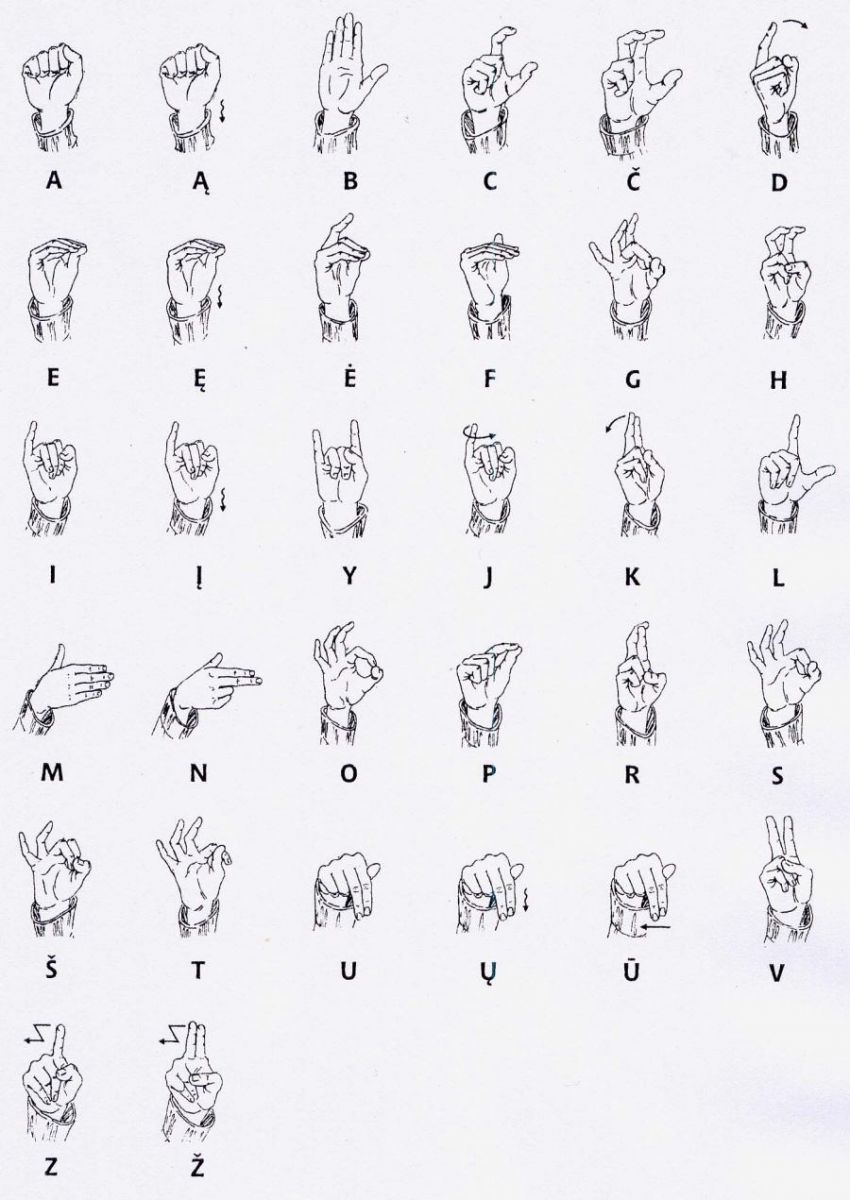
\includegraphics[width=.5\linewidth]{img/lsl_alphabet}
		\caption{Lietuvių gestų kalbos abėcėlė}
		\label{img:lsl_alphabet}
		%https://www.kspvm.lm.lt/images/naujienos/2016-2017/kurciuju-filmuko-laimejimas/img/lt-gestu-abecele.jpg
	\end{minipage}
\end{figure}

\subsection{Gestų kalbos atpažininimas}
Gestų kalba ir jos atpažinimas naudojant kompiuterinę techniką yra viena iš daugelio apsimokančių sistemų sričių. 

\subsubsection{Problematika}
Norint atpažinti gestus, paversti juos į žodžius ar sakinius susiduriama su problemomis, kurios susijusios tiek su statinių, tiek su dinaminių gestų atpažinimu.

Pagrindinės problemos iškylančios atpažįstant statinius gestų kalbos ženklus yra:
\begin{enumerate}
	\item Kiekvienos kalbos abėcėlę sudaro skirtingas raidžių (statinių ženklų) skaičius. \textit{Pavyzdžiui}, lietuvių kalbos abėcėlę sudaro 32 ženklai, o amerikietišką - 26; 
	\item Gestų panašumai. \textit{Pavyzdžiui}, raidės A, E, N, S, T yra atvaizduojamos sugniaužtus kumštį, o net trijose iš jų (A, E ir S) skiriasi tik nykščio padėtis;
	\item Kampas, kuris susidaro atpažįstant gestą. \textit{Pavyzdžiui}, kai A raidė rodoma ne iš priekio, o iš šono;
	\item Apšvietimas. \textit{Pavyzdžiui}, gestų atpažinimas esant prieblandai ir dienos šviesai.
\end{enumerate}

Pagrindinės problemos iškylančios atpažįstant dinaminius gestų kalbos ženklys yra:
\begin{enumerate}
	\item Nauji gestų kalbos žodžiai. \textit{Pavyzdžiui}, kiekvienas uraganas turi savo pavadinimą, todėl tai gali reikšti naujo gesto atsiradimą; 
	\item Gesto kelios reikšmės. \textit{Pavyzdžiui}, vienas gestas gali turėti kelias reikšmes, kaip kad lietuvių kalboje vienas žodis „kasa“ gali turėti net tris skirtingas reikšmes;
	\item Kampas, kuris susidaro atpažįstant gestą. \textit{Pavyzdžiui}, kai A raidė rodoma ne iš priekio, o iš šono;
	\item Žodžių apjungimas į vieną sakinį. \textit{Pavyzdžiui}, keli gestai einantys vienas po kito gali reikšti vieną žodį, tačiau tuo pačiu būti panašūs į vieną gestą, kuris jau reikš tik vieną žodį.
\end{enumerate}


Šiame skyriuje bus pateikta informacija, kaip atpažinti statinę gestų kalbą.

\section{Sistemos apmokymas}
Norint, jog sistema atpažintų gestus, svarbiausia ją apmokyti ką reiškia tam tikri gestai. Tam galime išnaudoti kadrus (\textit{angl. frame}) ir savaime apsimokančių sistemų galimybes. Tad reiktų imti vieną kadrą ir jį paversti į kompiuteriui suprantamą kalbą. 

Imkime, jog nuotrauka yra sudaryta iš \textit{n * m} taškų (\textit{angl. pixels}). Reikia, jog sistema atskirtų, kurioje kadro vietoje yra rodomo gesto dalis, kurioje tik pašalinis fonas.

Apmokymui toliau aptarsime Sobel valdiklį, savaime apsimokančių sistemų metodus ir duoemenų surinkimą 

\subsection{Sobel valdiklis}
\textbf{Sobel valdiklis} (\textit{angl. Sobel operator}) - vaizdų apdorojimo algoritmas, skirtas skirtas paversti kadrą į kontūrų žemėlapį.

Šis valdiklis naudojasi tokiomis operacijomis, kad konvertuotų vaizdą į kontūrus:

\begin{equation}\label{eq:sobelgx}
	G_x = 
	\begin{bmatrix}
	+1 & 0 & -1 \\
	+2 & 0 & -2 \\
	+1 & 0 & -1
	\end{bmatrix} * A
\end{equation}
	
\begin{equation}\label{eq:sobelgy}
	G_y = 
	\begin{bmatrix}
	+1 & +2 & +1 \\
	0 & 0 & 0 \\
	-1 & -2 & -1
	\end{bmatrix} * A
\end{equation}

\begin{equation}\label{eq:sobelg}
G = \sqrt{G_x^2 + G_y^2}
\end{equation}

\begin{figure}[H]
	\begin{minipage}{.3\textwidth}
		\centering
		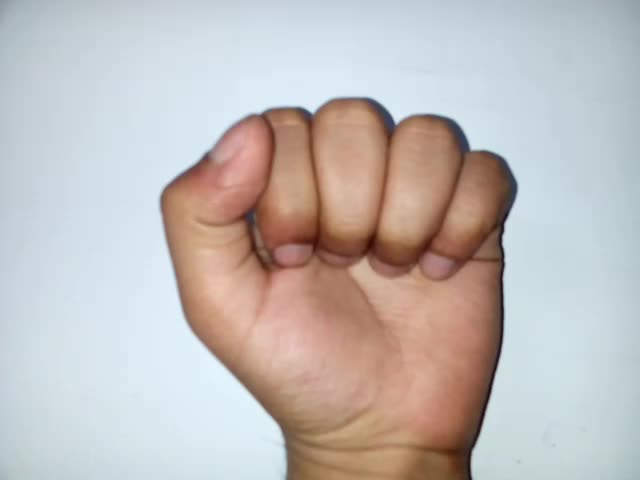
\includegraphics[width=.8\linewidth]{img/A}
		\caption{Orginalus paveikslėlis}
		\label{img:a-sign}
		%http://lifeprint.com/asl101/topics/wallpaper1.htm
	\end{minipage}\hspace{\fill}%
	\begin{minipage}{.3\textwidth}
		\centering
		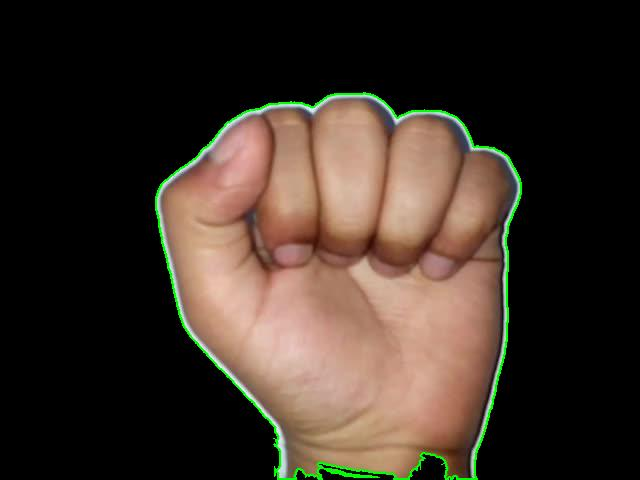
\includegraphics[width=.8\linewidth]{img/A-black}
		\caption{Be fono}
		\label{img:a-black-sign}
		%https://www.kspvm.lm.lt/images/naujienos/2016-2017/kurciuju-filmuko-laimejimas/img/lt-gestu-abecele.jpg
	\end{minipage}\hspace{\fill}%
	\begin{minipage}{.3\textwidth}
		\centering
		
\includegraphics[width=.8\linewidth]{img/A-white}
		\caption{Dviejų spalvų}
		\label{img:a-white-sign}
		%https://www.kspvm.lm.lt/images/naujienos/2016-2017/kurciuju-filmuko-laimejimas/img/lt-gestu-abecele.jpg
	\end{minipage}
\end{figure}
Kadras yra konvertuojamas į skaičių masyvą, kur kiekvienas taškas turi savo skaičių. Tuomet norint rasti visus kontūrus esančius kadre, taikome šiuos veiksmus:
\begin{enumerate}
	\item Einame per visus taškus esančius kadre ir taikydami \ref{eq:sobelgx} ir \ref{eq:sobelgy} formules, kur A - 3 x 3 kadro mastyvas;
	\item Įrašome gautąją reikšmę į dabartinį tašką;
	\item Apskaičiuojame dabartinio taško tikrąją reiškę taikydami \ref{eq:sobelg} formulę.
\end{enumerate}

Po šių žingsnių turime masyvą, kuris yra sudarytas iš reikšmių, esančių tarp 0 ir 255, kur 0 - juoda spalva, o 255 - balta. Taip, pritaikę savo kadrui gautą kaukę (\textit{angl. mask}) gauname kadrą, kuriame yra likę tik kontūrai(\textit{žr. \ref{img:a-black-sign} pav.})

Kitas žingsnis yra remiantis šia kauke paversti paveiksėlį į juodai baltą paveikslėlį (\textit{žr. \ref{img:a-white-sign} pav.}).

\subsection{Kadro atidavimas savaime apsimokančioms sistemoms}
Savaime apsimokančios sistemos, tokios kaip \textit{sklearn} konvertuoja jau apdorotą kadrą į matricą, kur juoda - 0, o balta - 255. Tuomet ši matrica yra „suplokštinama“ ir gauname masyvą. Galiausiai šiuos duomenis sudeda į failą, kad vėliau jais būtų galima pasinaudoti.


\section{Gestų kalbos statinių ženklų atpažinimas}
\subsection{Atpažinimas naudojant gestų nuotraukas}
Norint, jog sistema apsimokytų kuo tiksliau, reikia jai duoti kuo daugiau duomenų. Sakykime, kad:
\begin{itemize}
	\item\textit{a\textsubscript{ik}} - \textit{i}-toji \textit{k}-tosios abėcėlės raidės nuotrauka 
	\item\textit{a\textsubscript{1k}, a\textsubscript{2k}, ..., a\textsubscript{nk}} - nuotraukų rinkinys, sudarytas iš \textit{n} \textit{k}-tosios raidės nuotraukų
\end{itemize}
Tuomet, turėdami \textit{n * k} nuotraukų, kuriuose vaizduojami gestų abėcėlės gestai, turime, jog tiek eilučių duomenų turėsime gestams atpažinti. Kuo gestai yra įvairesni prie skirtingų apšvietimų, skirtingų rankų ir pan., tuo tiksliau sistema pati galės vėliau atpažinti gestus.


\subsection{Atpažinimas naudojant internetinę kamerą}
Norint atpažinti statinius gestus naudojant internetinę kamerą, vienas iš to būdų yra naudotis \textit{BackgroundSubtractorMOG2} klase. Ši klasė remiasi Gauso maišos priekinio plano/fono atskyrimo algoritmu


\section{Gestų kalbos dinaminių ženklų atpažinimas}


\section{Pagrindinė tiriamoji dalis}
Pagrindinėje tiriamojoje dalyje aptariama ir pagrindžiama tyrimo metodika;
pagal atitinkamas darbo dalis, nuosekliai, panaudojant lyginamosios analizės,
klasifikacijos, sisteminimo metodus bei apibendrinimus, dėstoma sukaupta ir
išanalizuota medžiaga.

\subsection{Poskyris}
Citavimo pavyzdžiai: cituojamas vienas šaltinis \cite{PvzStraipsnLt}; cituojami
keli šaltiniai \cite{PvzStraipsnEn, PvzKonfLt, PvzKonfEn, PvzKnygLt, PvzKnygEn,
PvzElPubLt, PvzElPubEn, PvzMagistrLt, PvzPhdEn}.

\subsubsection{Skirsnis}
\subsubsubsection{Straipsnis}
\subsubsection{Skirsnis}
\section{Skyrius}
\subsection{Poskyris}
\subsection{Poskyris}

\sectionnonum{Išvados}
Išvadose ir pasiūlymuose, nekartojant atskirų dalių apibendrinimų,
suformuluojamos svarbiausios darbo išvados, rekomendacijos bei pasiūlymai.

\printbibliography[heading=bibintoc] % Literatūros šaltiniai aprašomi
% bibliografija.bib faile. Šaltinių sąraše nurodoma panaudota literatūra,
% kitokie šaltiniai. Abėcėlės tvarka išdėstoma tik darbe panaudotų (cituotų,
% perfrazuotų ar bent paminėtų) mokslo leidinių, kitokių publikacijų
% bibliografiniai aprašai (šiuo punktu pasirūpina LaTeX). Aprašai pateikiami
% netransliteruoti.

\appendix  % Priedai
% Prieduose gali būti pateikiama pagalbinė, ypač darbo autoriaus savarankiškai
% parengta, medžiaga. Savarankiški priedai gali būti pateikiami kompiuterio
% diskelyje ar kompaktiniame diske. Priedai taip pat vadinami ir numeruojami.
% Tekstas su priedais siejamas nuorodomis (pvz.: \ref{img:mlp}).

\section{Niauroninio tinklo struktūra}
\begin{figure}[H]
    \centering
    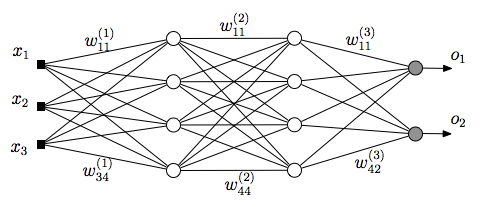
\includegraphics[scale=0.5]{img/MLP}
    \caption{Paveikslėlio pavyzdys}   % Antraštė įterpiama po paveikslėlio
    \label{img:mlp}
\end{figure}


\section{Eksperimentinio palyginimo rezultatai}
% tablesgenerator.com - converts calculators (e.g. excel) tables to LaTeX
\begin{table}[H]\footnotesize
  \centering
  \caption{Lentelės pavyzdys}    % Antraštė įterpiama prieš lentelę
  {\begin{tabular}{|l|c|c|} \hline
    Algoritmas & $\bar{x}$ & $\sigma^{2}$ \\
    \hline
    Algoritmas A  & 1.6335    & 0.5584       \\
    Algoritmas B  & 1.7395    & 0.5647       \\
    \hline
  \end{tabular}}
  \label{tab:table example}
\end{table}

\end{document}
